In h-multigrid, the different grids have the same polynomial order of finite elements but these elements are amalgamated into increasingly larger elements.
For LFA of h-multigrid, we introduce the concept of macro-element bases.
With macro-element bases, the grid transfer operators can be still represented elementwise and can thus be easily represented in the form of Equation \ref{eq:libceed_representation}.

A macro-element basis is formed by amalgamating two or more finite element bases.
Each sub-element has separate quadrature spaces, so the basis functions for each sub-element, are defined as zero on the portions of the domain not included in the given sub-element.
In effect, the basis interpolation and gradient operations for the macro-element provide a sub-element restriction and sub-element basis operation together.

\begin{figure}[!ht]
  \centering
  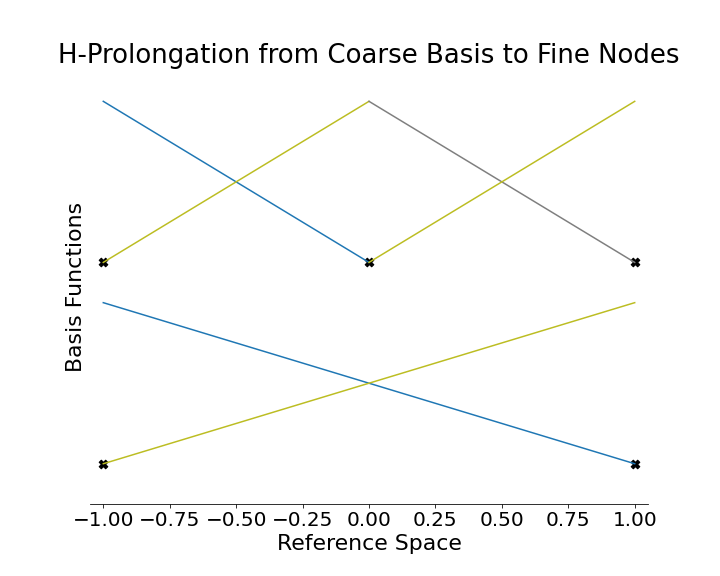
\includegraphics[width=0.48\textwidth]{../img/hProlongation}
  \caption{H-Prolongation from Coarse Basis to Fine Basis Points}
  \label{fig:h_prolongation}
\end{figure}

In Figure \ref{fig:h_prolongation}, we see an example of interpolation from a coarse grid basis to a fine grid macro-element basis.
The linear shape functions are evaluated at the nodes of the fine grid macro-element, which is a pair of linear sub-elements.
On the left linear sub-element, there are two basis functions which are zero over the domain of the right sub-element, and the reverse is also true.
The element level operator, ${\color{burgundy}\mathbf{A}}_e$, on the fine grid macro-element assembles the element level operator for each sub-element into the action of the PDE operator on the full macro-element.

With this macro-element structure, we can form the Fourier mode localization operator for the macro-element in the same fashion as the Fourier mode localization operator for high-order elements given in Equation \ref{eq:fouriermodelocalization1d}.
With macro-elements, there are $m p$ columns in the localization operator for a one dimensional scalar PDE on a macro-element with $m$ sub-elements instead of $p$ columns for a one dimensional scalar PDE on a single high order element.
\begin{equation}
\mathbf{Q} =
\begin{bmatrix}
    \mathbf{I}   \\
    \mathbf{e}_0 \\
\end{bmatrix} =
\begin{bmatrix}
    1      && 0      && \cdots && 0      \\
    0      && 1      && \cdots && 0      \\
    \vdots && \vdots && \vdots && \vdots \\
    0      && 0      && \cdots && 1      \\
    1      && 0      && \cdots && 0      \\
\end{bmatrix}
\end{equation}

Following the derivation from Section \ref{sec:lfahighorder}, we can derive the symbols of ${\color{burgundy}\mathbf{P}}_{\text{ctof}}$ and ${\color{burgundy}\mathbf{R}}_{\text{ftoc}}$.

\begin{definition}
The symbol of the h-prolongation operator is given by
\begin{equation}
\tilde{{\color{burgundy}\mathbf{P}}}_{\text{ctof}} \left( \boldsymbol{\theta} \right) = \mathbf{Q}_f^T \left( {\color{burgundy}\mathbf{P}}_e \odot \left[ e^{\imath \left( \mathbf{x}_{j, c} - \mathbf{x}_{i, f} \right) \cdot \mathbf{\theta} / \mathbf{h}} \right] \right) \mathbf{Q}_c
\end{equation}
where $i \in \left\lbrace 1, 2, \dots, n \left( m p + 1 \right)^d \right\rbrace$, $j \in \left\lbrace 1, 2, \dots, n \left( p + 1 \right)^d \right\rbrace$, $\mathbf{h}$ is the length of the macro-element, $d$ is the dimension of the finite element bases, $n$ is the number of components, and $m$ is the number of sub-elements in each fine grid macro-element.
The matrices $\mathbf{Q}_f$ and $\mathbf{Q}_c$ are the localization mappings for the fine and coarse grid, respectively, and the macro-element h-prolongation operator is given by ${\color{burgundy}\mathbf{P}}_e = {\color{blue(ncs)}\mathbf{I}} {\color{applegreen}\mathbf{D}}_{\text{scale}} {\color{blue(ncs)}\mathbf{B}}_{\text{ctof}}$.
\label{def:h_prolongation_symbol}
\end{definition}

\begin{definition}
The symbol of h-restriction operator is given by the expression
\begin{equation}
\tilde{{\color{burgundy}\mathbf{R}}}_{\text{ftoc}} \left( \boldsymbol{\theta} \right) = \mathbf{Q}_c^T \left( {\color{burgundy}\mathbf{R}}_e \odot \left[ e^{\imath \left( \mathbf{x}_{j, f} - \mathbf{x}_{i, c} \right) \cdot \boldsymbol{\theta} / \mathbf{h}} \right] \right) \mathbf{Q}_f
\end{equation}
where $i \in \left\lbrace 1, 2, \dots, n \left( p + 1 \right)^d \right\rbrace$, $j \in \left\lbrace 1, 2, \dots, n \left( m p + 1 \right)^d \right\rbrace$, $\mathbf{h}$ is the length of the macro-element, $d$ is the dimension of the finite element bases, $n$ is the number of components, and $m$ is the number of sub-elements in each fine grid macro-element.
The matrices $\mathbf{Q}_f$ and $\mathbf{Q}_c$ are the localization mappings for the fine and coarse grid, respectively, and the macro-element h-restriction operator is given by ${\color{burgundy}\mathbf{R}}_e = {\color{burgundy}\mathbf{P}}_e^T = {\color{blue(ncs)}\mathbf{B}}_{\text{ctof}}^T {\color{applegreen}\mathbf{D}}_{\text{scale}} {\color{blue(ncs)}\mathbf{I}}$.
\label{def:h_restriction_symbol}
\end{definition}

\begin{figure}[!ht]
  \centering
  \subfloat[Spectrum of H-Multigrid for $p = 1$]{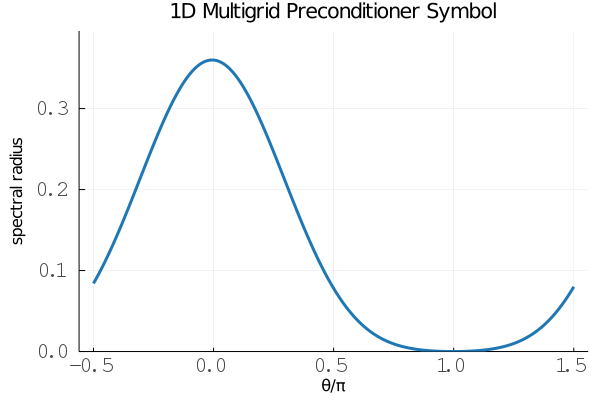
\includegraphics[width=0.48\textwidth]{../img/hmultigridSymbol1D}\label{fig:h_multigrid_spectrum_1d}}
  \hfill
  \subfloat[Spectrum of H-Multigrid for $p = 1$]{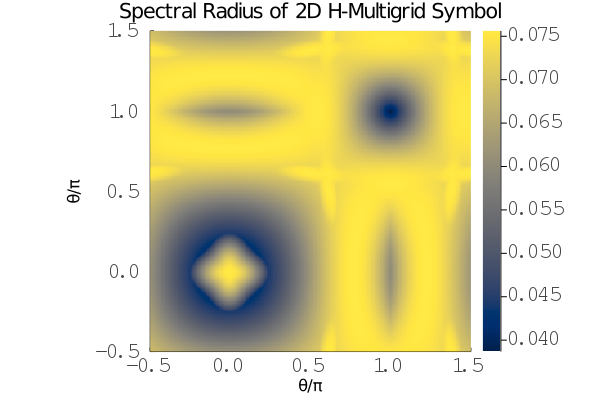
\includegraphics[width=0.48\textwidth]{../img/hmultigridSymbol2D}\label{fig:h_multigrid_spectrum_2d}}
  \caption{Spectrum of Spectrum of H-Multigrid Symbol for $p = 1$}
\end{figure}

In Figures \ref{fig:h_multigrid_spectrum_1d} and \ref{fig:h_multigrid_spectrum_2d}, we see the spectral radius of the symbol of h-multigrid for the scalar diffusion operator with third-order Chebyshev smoothing on a fine grid with a fourth-order H1 Lagrange finite element basis and a coarse grid with a second-order H1 Lagrange finite element basis on the Gauss-Lobatto points in one and two dimensions.
Various preconditioning techniques will reduce this spectral radius, with different effectiveness in different frequency ranges.

% -----------------------------------------------------------------------------
\subsection{H-Multigrid Validation with Previous Work}
% -----------------------------------------------------------------------------

By representing the fine grid with macro-elements and the prolongation operator with this interpolation, this LFA of p-multigrid exactly reproduces the results of He and Maclachlan \cite{he2020two} for LFA of high-order h-multigrid even though this previous work did not use the concept of macro-elements.
The results from this LFA can be seen in Table \ref{table:two_grid_hmultigrid}.

\begin{table}[ht!]
\begin{center}
\begin{tabular}{l cc cc cc}
  \toprule
  $p, d$  &  \multicolumn{2}{c}{$\nu = \left( 0, 1 \right)$}  &  \multicolumn{2}{c}{$\nu = \left( 1, 1 \right)$}  &  \multicolumn{2}{c}{$\nu = \left( 2, 2 \right)$}  \\
  %\cmidrule(lr){2-3} \cmidrule(lr){4-5} \cmidrule(lr){6-7}
                      &  $\rho$  &  $\omega$  &  $\rho$ & $\omega$  &  $\rho$ & $\omega$  \\
  \toprule
  $p = 2, d = 1$  &  0.821 & 1.000  &  0.821 & 1.000  &  1.279 & 1.000   \\
  $p = 2, d = 1$  &  0.526 & 0.838  &  0.495 & 0.838  &  0.302 & 0.838   \\
  $p = 2, d = 1$  &  0.291 & 0.709  &  0.249 & 0.709  &  0.064 & 0.709   \\
  \midrule
  $p = 3, d = 1$  &  0.491 & 0.650  &  0.337 & 0.650  &  0.131 & 0.650   \\
  \midrule
  $p = 4, d = 1$  &  0.608 & 0.640  &  0.559 & 0.640  &  0.331 & 0.640   \\
  \midrule
  $p = 2, d = 2$  &  0.452 & 1.000  &  0.288 & 1.000  &  0.091 & 1.000   \\
  \bottomrule
\end{tabular}
\end{center}
\caption{Two-grid convergence factor and Jacobi smoothing parameter for high-order h-multigrid}
\label{table:two_grid_hmultigrid}
\end{table}

On uniform rectangular meshes, linear finite elements produce the same discetized operator as finite differencing.
The nine-point stencil for the Laplace operator in 2D is given by

\begin{equation}
\frac{1}{3}
\begin{bmatrix}
-1  &  -1  &  -1   \\
-1  &   8  &  -1   \\
-1  &  -1  &  -1  \\
\end{bmatrix}
\end{equation}
with a corresponding local Fourier analysis symbol given by

\begin{equation}
\tilde{A} \left( \theta_1, \theta_2 \right) = \frac{8}{3} - \frac{2}{3} \cos \left( \theta_1 \right) - \frac{2}{3} \cos \left( \theta_2 \right) - \frac{4}{3} \cos \left( \theta_1 \right) \cos \left( \theta_2 \right)
\end{equation}

The assembled matrix for a single linear element is given by

\begin{equation}
{\color{burgundy}\mathbf{A}}^e =
\frac{1}{3}
\begin{bmatrix}
 2    &  -1/2  &  -1/2  &  -1    \\
-1/2  &   2    &  -1    &  -1/2  \\
-1/2  &  -1    &   2    &  -1/2  \\
-1    &  -1/2  &  -1/2  &   2    \\
\end{bmatrix}
\end{equation}
with a corresponding local Fourier analysis symbol given by

\begin{equation}
\begin{split}
\tilde{\color{burgundy}\mathbf{A}} \left( \theta_1, \theta_2 \right) & = \mathbf{Q}^T \left( {\color{burgundy}\mathbf{A}}^e \odot \left[ e^{\imath \left( \mathbf{x}_j - \mathbf{x}_i \right) \cdot \boldsymbol{\theta}} \right] \right) \mathbf{Q}\\ & = \frac{8}{3} - \frac{2}{3} \cos \left( \theta_1 \right) - \frac{2}{3} \cos \left( \theta_2 \right) - \frac{4}{3} \cos \left( \theta_1 \right) \cos \left( \theta_2 \right).
\end{split}
\end{equation}

We can use the LFA of multigrid given by Definition \ref{def:multigrid_symbol} with the symbols of the h-multigrid transfer operators givn by Definition \ref{def:h_prolongation_symbol} and Definition \ref{def:h_restriction_symbol} to reproduce LFA of h-multigrid methods for finite differencing where the stencil can be represented by a finite element discretization.
This LFA of arbitrary second-order PDEs with high-order finite element discretizations agrees with previous work on LFA of PDE operators derived with finite differencing with analogus stencils.

Our LFA of h-multigrid presented here is based on a specific basis of the Fourier space used in \cite{kumar2019local} rather than the commonly used Fourier modes, see \cite{MR1807961,wienands2004practical}, where the symbol of each component in multigrid methods are formed based on different harmonic frequencies.
The symbols of grid-transfer operators described in Definition \ref{def:h_prolongation_symbol} and Definition \ref{def:h_restriction_symbol} give a general way for multigrid coarsening with factor $m$, and this framework is simpler, especially for high-order discretizations described in \cite{he2020two}.
Also, our LFA for h-multigrid is suitable for finite element discretizations without requiring bases to have uniformly spaced nodes.

As mentioned before, our focus of this work is p-multigrid, so we will not expand the discussion of h-multigrid further method here.
Applying this LFA framework to h-multigrid or hp-multigrid methods are topics for future research.
